%% LyX 1.3 created this file.  For more info, see http://www.lyx.org/.
%% Do not edit unless you really know what you are doing.
\documentclass[english, 12pt]{article}
\usepackage{times}
%\usepackage{algorithm2e}
\usepackage{url}
\usepackage{bbm}
\usepackage[T1]{fontenc}
\usepackage[latin1]{inputenc}
\usepackage{geometry}
\geometry{verbose,letterpaper,tmargin=2.5cm,bmargin=2.5cm,lmargin=2.5cm,rmargin=2.5cm}
\usepackage{rotating}
\usepackage{color}
\usepackage{graphicx}
\usepackage{amsmath, amsthm, amssymb}
\usepackage{setspace}
\usepackage{lineno}
\usepackage{hyperref}
\usepackage{bbm}

\linenumbers
\doublespacing
%\usepackage[authoryear]{natbib}
\usepackage{natbib} \bibpunct{(}{)}{;}{author-year}{}{,} 

%Pour les rajouts
\usepackage{color}
\definecolor{trustcolor}{rgb}{0,0,1}

\usepackage{dsfont}
\usepackage{adjustbox}
\usepackage{multirow}
\usepackage{graphicx}
\graphicspath{{../figures/}}
\DeclareMathOperator*{\argmin}{\arg\!\min}

\let\tabbeg\tabular
\let\tabend\endtabular
\renewenvironment{tabular}{\begin{adjustbox}{max width=\textwidth}\tabbeg}{\tabend\end{adjustbox}}

\makeatletter

%%%%%%%%%%%%%%%%%%%%%%%%%%%%%% LyX specific LaTeX commands.
%% Bold symbol macro for standard LaTeX users
%\newcommand{\boldsymbol}[1]{\mbox{\boldmath $#1$}}

%% Because html converters don't know tabularnewline
\providecommand{\tabularnewline}{\\}

\usepackage{babel}
\makeatother


\begin{document}


\title{Predicting complex diseases: performance and robustness}
\author{Florian Priv�\,$^{\text{ 1,}*}$, Hugues Aschard\,$^{\text{2,3}}$ and Michael G.B. Blum\,$^{\text{1,}*}$}



\date{~ }
\maketitle

\noindent$^{\text{\sf 1}}$Universit� Grenoble Alpes, CNRS, Laboratoire TIMC-IMAG, UMR 5525, France, \\
\noindent$^{\text{\sf 2}}$Centre de Bioinformatique, Biostatistique et Biologie Int�grative (C3BI), Institut Pasteur, Paris, France \\
\noindent$^{\text{\sf 3}}$Department of Epidemiology, Harvard T.H. Chan School of Public Health, Boston, Massachusetts, USA.

\noindent$^\ast$To whom correspondence should be addressed.

\newpage
\abstract{
\textbf{Motivation:} \\
\textbf{Results:} \\
\textbf{Availability:} \\
\textbf{Contact:} \href{florian.prive@univ-grenoble-alpes.fr}{florian.prive@univ-grenoble-alpes.fr} \& \href{michael.blum@univ-grenoble-alpes.fr}{michael.blum@univ-grenoble-alpes.fr}\\
\textbf{Supplementary information:}
}

\newpage
\section{Introduction}

Polygenic Risk Scores (PRSs) combine the information contained in many single-nucleotide polymorphisms (SNPs) in a score that should reflect the risk of developing diseases. PRSs have proven to be useful for different applications, such as finding a common genetic contribution between two diseases [@Purcell2009]. 
Personalized medicine is one of the major applications of PRSs. Personalized medicine will use PRSs in screening campains in order to identify people at higher risk for a given disease. ...This could lead to prevention for these identified people...
Personalized medicine with also use PRSs for helping in the diagnostic of disease, either confirming a diagnostic or even early diagnostic. Yet, diagnostic based on PRSs won't be possible unless these PRSs shows a high discrimitative power between cases and controls [REF].
Many methods have been developed in order to maximize the predictive power of genotypes for diseases, or more generally phenotypes.
A commonly used technique, called P+T (which stands for ``Pruning + Thresholding'') or genetic profiling, is used to derive a PRS from results of Genome-Wide Association Study (GWAS). This technique only use summary statistics which make it very ..suitable.. and also very fast.
Linear Mixed-Models are also widely-used in fields such as plant and animal breeding or for predicting highly heritable quantitative human phenotypes such as height [REF]. Yet, these models are not ..constructed.. for predicting a binary trait such as a disease and have proven to ..fail.. at such in another comparative study [REF GAD]. Moreover, these methods and their derivations are often computationally demanding and won't be usable for largest cohorts to data [REFS].
Statistical learning methods such as logistic regression, Support Vector Machine (SVM) or random forests were also used to derive PRSs for complex human disease by jointly estimating SNP effects.

We recently developed two R packages, bigstatsr and bigsnpr, for efficient management and analysis of large-scale genome-wide data. This include efficient functions for computing penalized linear and logistic regressions on huge datasets. In this paper, we present a comprehensive analysis of the P+T method, our penalized logistic regression and the T-Trees algorithm, which is a derivation of random forests and has given exceptionally good results in its corresponding paper [REF BOTTA]. Note that SVM is expected to give similar results to logistic regression [REF GAD], and therefore isn't added to the comparison.
For the P+T model, we compare different threshold of inclusion of SNPs, as it has been a burning question for some years.
For the logistic regression, we include two novel approaches. First, we introduce a procedure that we call Cross-Model Selection and Averaging (CMSA) for ``choosing'' the optimal threshold of inclusion of SNPs. We also show how easy it is to tweak the method in order to capture not only linear effects, but also recessive/dominant effects.
Finally, we quickly discard T-Trees as being a suitable method for predicting disease status based on genotypes.
In order to make our comparison as comprehensive as possible, we compare different architectures of disease (number, size and location of causal effects and heritability) with different model of generating liability ..scores.., one with only linear effects, and one which combine linear, recessive, dominant and interaction effects. 

We show that penalized logistic regression consistently performs better than the P+T method whereas predictive performance of the P+T method is very sensitive to the threshold of inclusion of SNPs [MONTRER UN GRAPH EN FCT D'INCLUSION].

\section{Methods}

\subsection{Simulations} \label{sec:simus}

For simulations, we use real genotypes of European individuals from a case/control celiac disease cohort [REF]. 
This dataset has been quality-controled and imputed in another study [REF MOI].
To get rid of the structure induced by the celiac disease, we keep only controls from this cohort. Moreover, to get rid of population structure, we keep only people from UK and further subset these British people based on deviation of Robust Mahalanobis distance on Principal Components (see ..SupMat..), leaving 7102 individuals genotypes on ..28x,xxx.. SNPs [ADD DIM TO RMD] with minimal population structure (see ..SupMat..) because this....

To simulate phenotypes, we use a the Liability Threshold Model (LTM) with a prevalence of 30\%. We vary different parameters: the number of causal variants and their location (30, 300 or 3000 anywhere in the genome and 30 only in the HLA region), the heritability (0.5 or 0.8), the distribution of effects associated with causal SNPs (Normal or Laplace), and the model used to generate the genetic ..part.. of the phenotypes (one with only linear effects, and one which combine linear, recessive, dominant and interaction effects). This simulation is broader yet similar to the one used in [REF STEPHENS]. 

For the ``simple model'', we compute $$y_i = \sum_{j\in E_\text{causal}} w_j \cdot \widetilde{G_{i,j}}$$ where $w_j$ are weights ($w_j \neq 0$ if and only if SNP $j$ is causal), $G_{i,j}$ is the allele count of individual $i$ for SNP $j$ and $\widetilde{G_{i,j}}$ corresponds to its standardized version (zero mean and unit variance for all SNPs). \\
For the ``fancy model'', we separate the causal SNPs in three equal sets $E_\text{causal}^{(1)}$, $E_\text{causal}^{(2)}$ 
and $E_\text{causal}^{(3)}$ ($E_\text{causal}^{(3)}$ is further separated in two equal sets, $E_\text{causal}^{(3.1)}$ and $E_\text{causal}^{(3.2)}$) 
and we compute $$y_i = \underbrace{\sum_{j\in E_\text{causal}^{(1)}} w_j \cdot \widetilde{G_{i,j}}}_\text{linear} + \underbrace{\sum_{j\in E_\text{causal}^{(2)}} w_j \cdot \widetilde{D_{i,j}}}_\text{recessive/dominant} + \underbrace{\sum_{\substack{k=1 \\ j_1=e_k^{(3.1)} \\ j_2=e_k^{(3.2)}}}^{k=\left|E_\text{causal}^{(3.1)}\right|} w_{j_1} \cdot \widetilde{G_{i,j_1} \cdot G_{i,j_2}}}_\text{interaction}$$ where $D_{i,j} = \mathds{1}\left\{G_{i,j} \neq 0\right\}$ and $E_\text{causal}^{(q)}=\left\{e_k^{(q)}, k \in \left\{1, \ldots, \left|E_\text{causal}^{(q)}\right|\right\}\right\}$. Note that for the interaction part of the model, we scale interactions, not the raw allele counts, so that corresponding SNPs still display a marginal effect. \\
For both models, the $y_i$ are then standardized such that they have a variance equal to the desired heritability $h^2$ and we further add some environmental noise $\epsilon_i$ to $y_i$ where $\epsilon \sim N(0, 1 - h^2)$.

This results in 32 combinations of parameters and we run 100 simulations for each of these combinations (5 times more than in [REF STEPHENS]), resulting of a total of 3200 simulations. For each of these 3200 simulations, we randomly re-sample a training set of 6000 individuals, with the corresponding test set composed of the remaining individuals.


\subsection{Predictive performance measures}

In this study, we use two different measures of predictive accuracy. 
First, we use the Area Under the Receiver Operating Characteristic (ROC) Curve (AUC). In the case of our study, the AUC is the probability that a PRS of a case is greater than one of a control.
This measure indicates how well we can distinguish between cases and controls using PRSs.
As a second measure, we report the percentage of cases in the 10\% largest PRSs [UTILISER 20\%?]. This measure indicates how well we can identify people at higher risk from a higher PRS in screening campaigns.

Note that we also report the timing of the main computations and the number of SNPs used for the prediction.

\subsection{Compared methods}

In this study, we compare three different types of methods: the P+T method, the T-Trees method and a penalized logistic regression.

The P+T (Pruning + Thresholding) method directly derives a Polygenic Risk Score (PRS) from the results of Genome-Wide Associations Studies (GWASs) that are commonly called summary statistics.
For the P+T method, a coefficient of regression is learned independently for each SNP along with a corresponding p-value (the GWAS part). GWAS was performed using logistic regressions, with 10 first Principal Components (PCs) as covariates in the models.
The SNPs are first clumped (P) so that there remains only loci that are weakly correlated with each other. 
Thresholding (T) consists in removing SNPs that are under a certain level of significance (P-value threshold to be determined). 
Finally, a polygenic risk score is defined as the sum of allele counts of the remaining SNPs weighted by the corresponding effect coefficients: $$S_i = \sum_{j \in E_\text{clumping}} \mathds{1}\{p_j < T\} \cdot \beta_j \cdot G_{i,j}$$ where $\beta_j$ ($p_j$) are the effect sizes (p-values) learned from the GWAS and $T$ is a threshold to be determined. In this study, we report scores for a clumping threshold at $r^2 > 0.2$ with regions of 500kb. [threshold in results?]
[DIRE CA??:] All these steps are implemented in R packages bigstatsr and bigsnpr [REF MOI].

T-Trees (\textit{Trees inside Trees}) is an algorithm derived from random forests [REF 2001, BReiman] that takes into account the correlation structure among the genetic markers implied by linkage disequilibrium in GWAS data [REF BOTTA]. In a previous study on WTCCC data [REF], it achieved too-good-to-be-true results. Since this method is significantly different from the other tested here, we decided to include it in this comparison in order to assess whether or not it could give superior predictive performance. We use the same parameters as reported in Table 4 of the T-Trees paper, yet, we use only 100 trees (instead of 1000) because it showed only a very subtle increase of AUC while taking way too much time (e.g. AUC of 81.5\% instead of 81\%, data not shown).


The last method we compare is penalized logistic regression.
We solve: $$\argmin_{\beta_0, \beta}(x, y, \lambda)\left\{\underbrace{\frac{1}{n}\sum_{i=1}^n \log\left(1+e^{-y_i (\beta_0+x_i^T\beta)}\right)}_\text{Loss function} + \underbrace{\lambda \left((1-\alpha)\frac{1}{2}\|\beta\|_2^2 + \alpha \|\beta\|_1\right)}_\text{Penalization}\right\}$$ where, in this study, $x$ is the genotypes and covariables (e.g. PCs), $y$ is disease status we want to predict and $\lambda$ is a regularization parameter that need to be determined. 
Different regularizations can be used to prevent overfitting, among other benefits: the L2-regularization (ridge, @Hoerl1970) shrinks coefficients and is ideal if there are many predictors drawn from a Gaussian distribution (corresponds to $\alpha = 0$),
 the L1-regularization (lasso, @Tibshirani1996) forces some of the coefficients to be exactly zero and can be used as a means of variable selection, leading to sparse (and therefore more interpretable) models  (corresponds to $\alpha = 1$), 
the L1- and L2-regularization (elastic-net, @Zou2005) is a compromise between the two previous penalties and is particularly useful in the $m \gg n$ situation, or any situation where there are many correlated predictors (corresponds to $0 < \alpha < 1$) (@Friedman2010). In this study, we always use $\alpha = 0.5$, without trying to tune the value of this hyper-parameter $\alpha$ (e.g. by grid-search and cross-validation).

To fit this penalized logistic regression, we use a very efficient algorithms based on (@Friedman2010, ...2012 and biglasso...), also implemented in our package bigstatsr. This type of algorithms build predictions for many values of $\lambda$ (typically 100). To get an algorithm free of the choice of this hyper-parameter $\lambda$, we developed a procedure that we called Cross-Model Selection and Averaging (CMSA). First, this method separates the training set in $K$ folds (e.g. 10). Secondly, in turn, each fold is considered as an inner validation set and the others ($K - 1$) folds form an inner training set, the model is trained on the inner training set and the corresponding predictions (scores) for the inner validation set are computed, the vector of scores which maximizes a criterion (e.g. AUC) is determined and the vector of coefficients corresponding to the previous vector of scores is chosen. Finally, the $K$ resulting vectors of coefficients are then combined into one vector (e.g. using the geometric median). Because of L1-regularization, this vector of coefficients is typically very sparse and can be used to make a PRS based on a linear combination of allele counts.

\subsection{Reproduciblity}

All the code used in this paper along with results,  such as execution times and figures,  are available as HTML R notebooks in the Supplementary Materials.

\section{Results}

\subsection{Overview and naming}

\subsection{T-Trees}

First, we ran only 5 simulations for each combination of parameters (see section \ref{sec:simus}), excepted for the heritability that we fixed at $0.8$.
The goal was to quickly discard the T-Trees method as being competitive with the other methods. 
For example, compared to our penalized logistic regression, T-Trees perform worse for both predictive measures, the AUC and the percentage of cases in highest scores. Moreover, T-Trees takes longer to run and makes more complex predictive models because it uses more SNPs in the models and have non-linear effects (Figure \ref{fig:ttrees}).
So, we decided to discard this method for the rest of the simulations.

\subsection{Main simulations}

For the P+T method, we report three different scores of prediction: one including all the SNPs (after clumping), one including only SNPs that have a p-value under the GWAS threshold of significance ($p < 5 \cdot 10^{-8}$), and one that maximize the AUC for these two thresholds and a sequence of 100 values from $10^{-0.1}$ to $10^{-100}$ equally spaced on the log-log-scale (Table \ref{tab:thr}). Note that, normally, the optimal threshold would have to be learned on the training set only. We consider this reported maximum AUC as an upper bound of the AUC for the P+T method.

[Also return p-values?]

[TIMING: PRS -> 0; logit -> 500-600 with small increase when more causal variants, logit-triple x3]

[AUC: decrease with M, PRS-all never good, logit-triple better for fancy and almost as good for simple]

[\% Cases: Linear with AUC, Attention perc cases is == 30%] 



\section{Discussion}


\newpage
\section*{Acknowledgements}

Authors acknowledge Grenoble Alpes Data Institute, supported by the French National Research Agency under the ``Investissements d?avenir'' program (ANR-15-IDEX-02) and the LabEx PERSYVAL-Lab (ANR-11-LABX-0025-01).

\vspace*{-12pt}

\bibliographystyle{natbib}
\bibliography{document}

\newpage
\section*{Supplementary Data}

\renewcommand{\thefigure}{S\arabic{figure}}
\setcounter{figure}{0}
\renewcommand{\thetable}{S\arabic{table}}
\setcounter{table}{0}

\begin{figure}[h]
\centerline{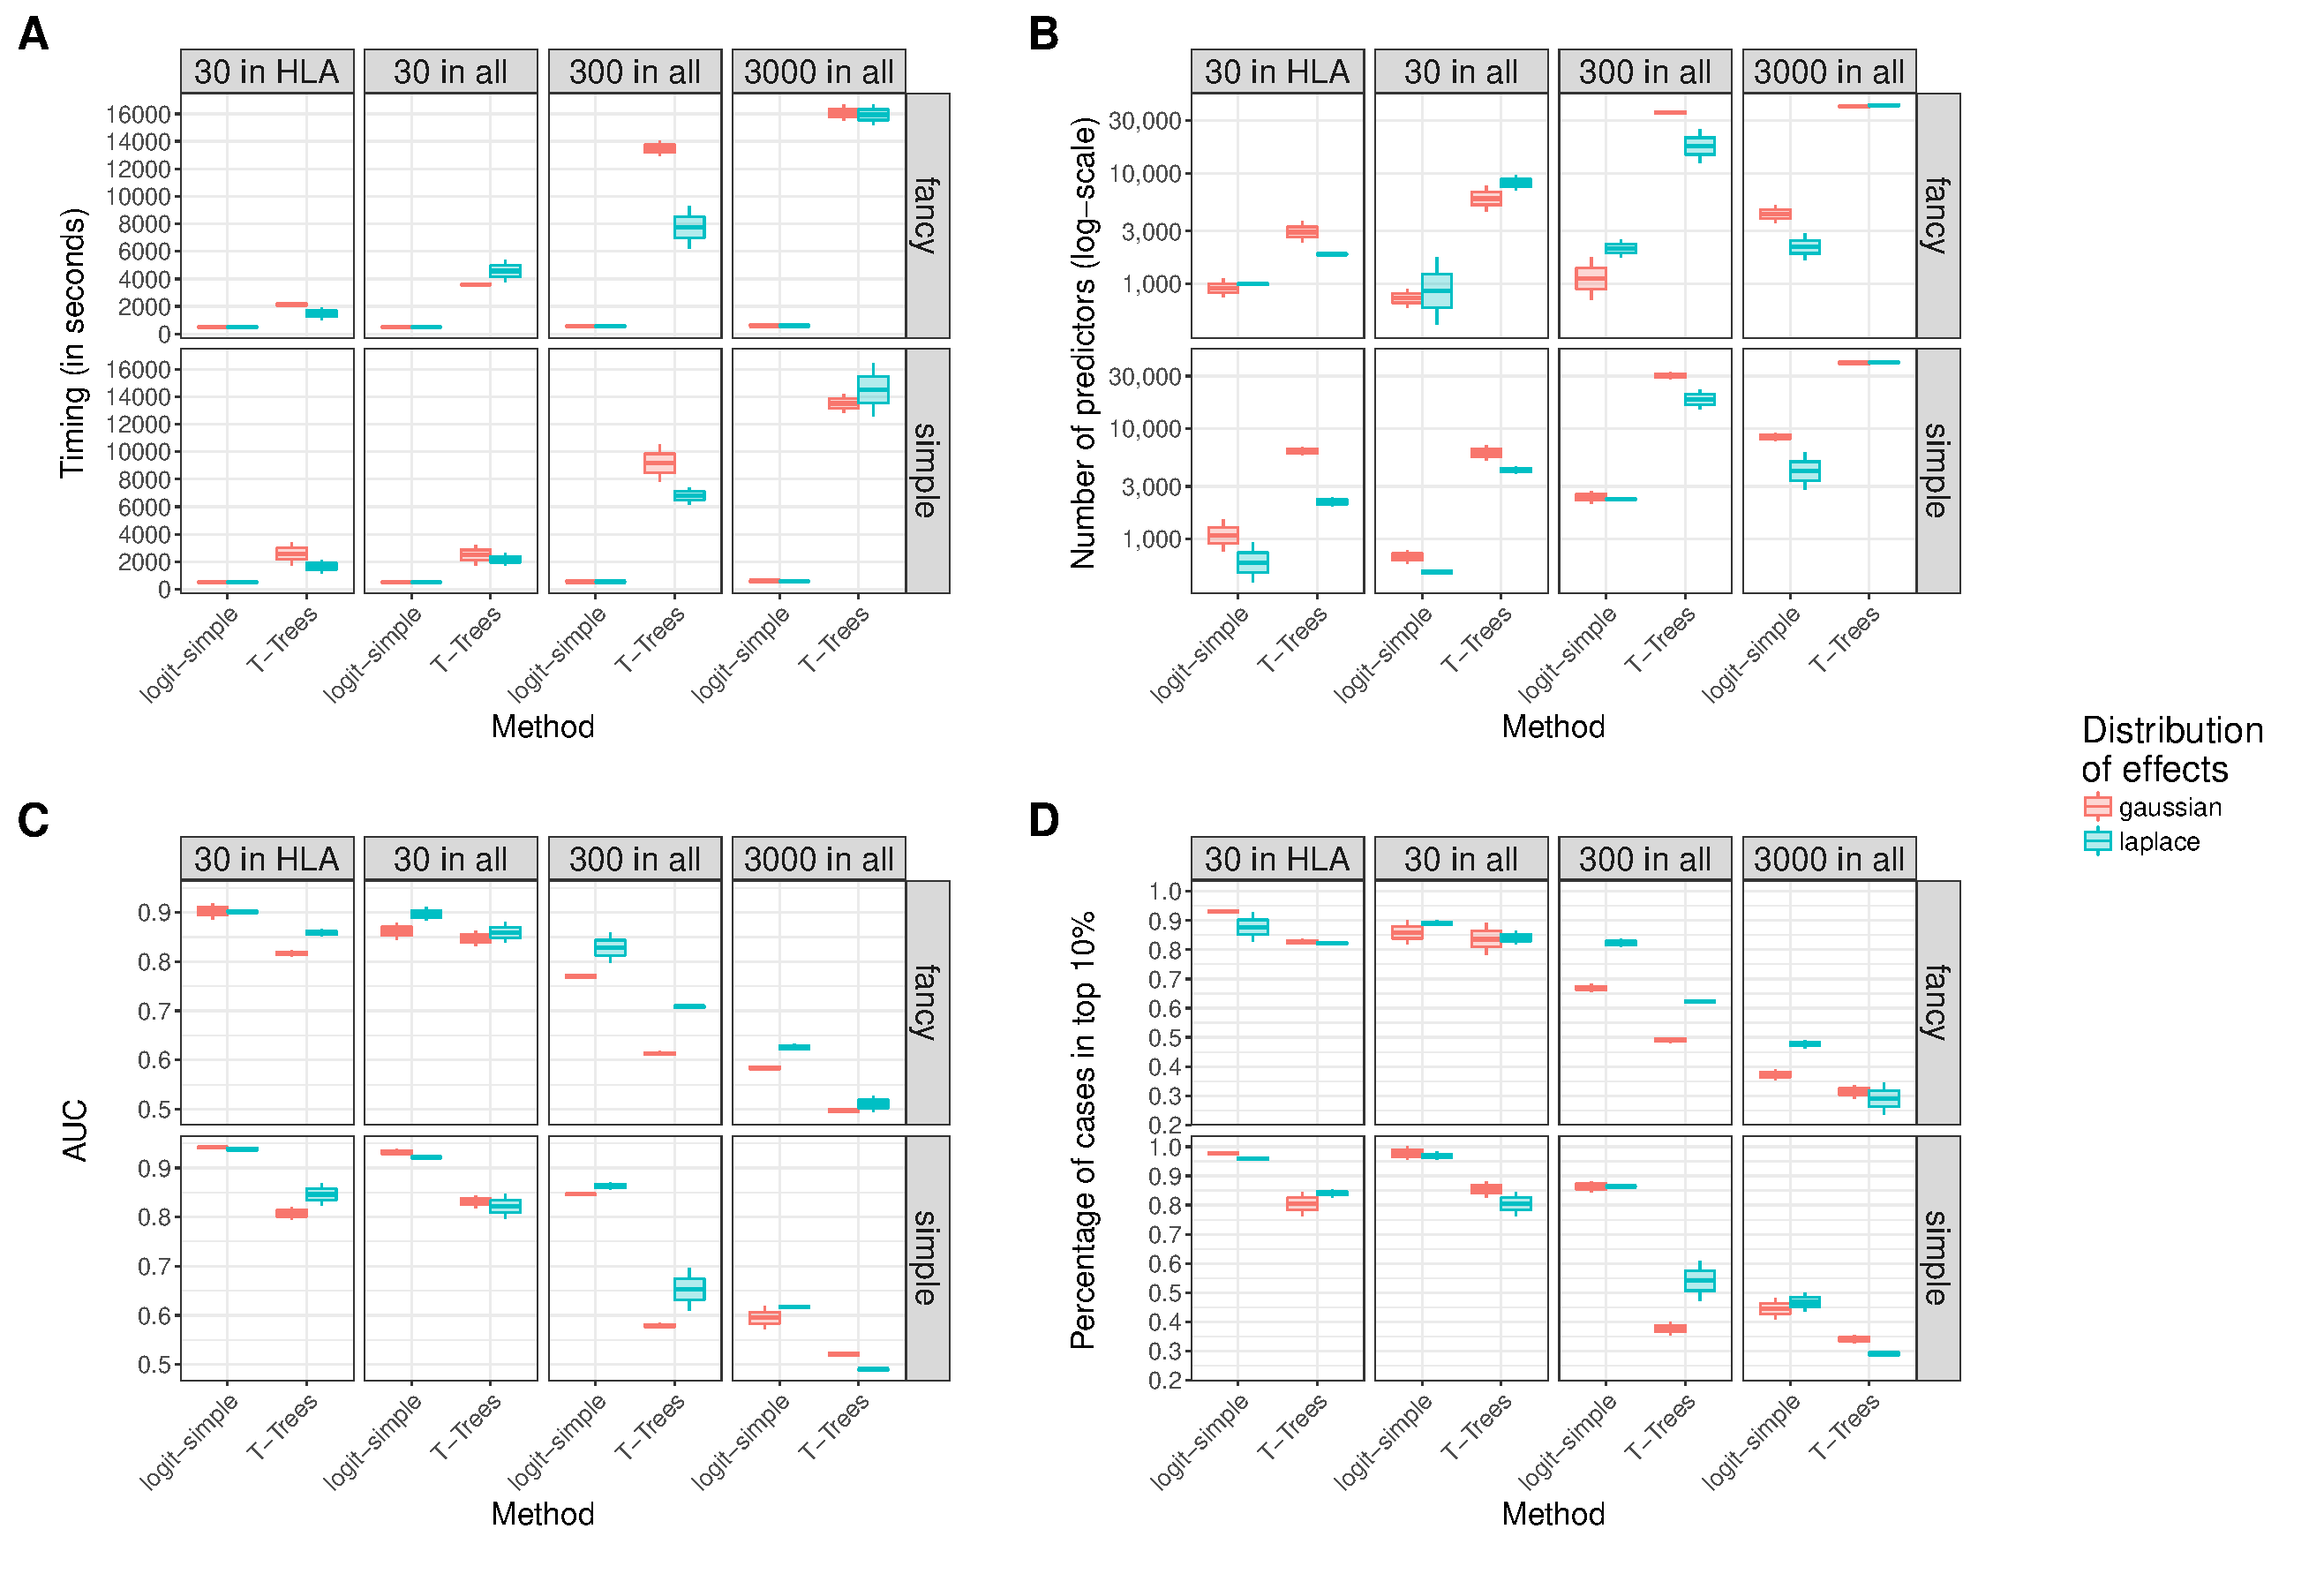
\includegraphics[width=\textwidth]{ttrees}}
\caption{Results of T-Trees vs penalized logistic regression. \textbf{A.} Timing (in seconds). \textbf{B.} Number of predictors of the model. \textbf{C.} AUC. \textbf{D.} Percentage of cases in the 10\% largest scores.}\label{fig:ttrees}
\end{figure}

% latex table generated in R 3.4.1 by xtable 1.8-2 package
% Thu Oct 26 16:46:26 2017
\begin{table}[ht]
\centering
\begin{tabular}{ccccccccccccccc}
  \hline
1.00e+00 & 7.22e-01 & 5.87e-01 & 4.20e-01 & 2.43e-01 & 1.00e-01 & 2.35e-02 & 2.21e-03 & 4.69e-05 & 8.81e-08 & 3.18e-12 & 1.83e-19 & 2.89e-31 & 1.70e-50 & 7.71e-82 \\ 
  5.00e-08 & 7.05e-01 & 5.65e-01 & 3.95e-01 & 2.20e-01 & 8.47e-02 & 1.79e-02 & 1.42e-03 & 2.28e-05 & 2.73e-08 & 4.69e-13 & 8.08e-21 & 1.80e-33 & 4.30e-54 & 1.06e-87 \\ 
  7.94e-01 & 6.87e-01 & 5.42e-01 & 3.69e-01 & 1.97e-01 & 7.08e-02 & 1.34e-02 & 8.83e-04 & 1.05e-05 & 7.74e-09 & 6.03e-14 & 2.86e-22 & 7.73e-36 & 5.97e-58 & 5.49e-94 \\ 
  7.81e-01 & 6.69e-01 & 5.19e-01 & 3.43e-01 & 1.75e-01 & 5.85e-02 & 9.79e-03 & 5.31e-04 & 4.61e-06 & 2.01e-09 & 6.69e-15 & 7.92e-24 & 2.24e-38 & 4.37e-62 & 1.00e-100 \\ 
  7.67e-01 & 6.50e-01 & 4.95e-01 & 3.18e-01 & 1.54e-01 & 4.76e-02 & 7.01e-03 & 3.08e-04 & 1.90e-06 & 4.72e-10 & 6.32e-16 & 1.70e-25 & 4.26e-41 & 1.61e-66 &  \\ 
  7.53e-01 & 6.30e-01 & 4.70e-01 & 2.93e-01 & 1.35e-01 & 3.82e-02 & 4.90e-03 & 1.72e-04 & 7.31e-07 & 1.00e-10 & 5.04e-17 & 2.75e-27 & 5.16e-44 & 2.83e-71 &  \\ 
  7.38e-01 & 6.09e-01 & 4.46e-01 & 2.68e-01 & 1.17e-01 & 3.02e-02 & 3.33e-03 & 9.18e-05 & 2.63e-07 & 1.89e-11 & 3.35e-18 & 3.31e-29 & 3.84e-47 & 2.26e-76 &  \\ 
   \hline
\end{tabular}
\caption{The 102 thresholds used in the P+T method for this study.}
\label{tab:thr}
\end{table}

\end{document}
